\documentclass{article}
\usepackage[utf8]{inputenc}
\usepackage[spanish]{babel}
\usepackage{listings}
\usepackage{graphicx}
\usepackage{hyperref}
\graphicspath{ {images/} }
\usepackage{cite}

\begin{document}

\begin{titlepage}
    \begin{center}
        \vspace*{1cm}
            
        \Huge
        \textbf{Nociones de la memoria del computador}
            
        \vspace{0.5cm}
        \LARGE
        Proyecto de investigación
            
        \vspace{1.5cm}
            
        \textbf{Angie Paola Jaramillo Ortega}
            
        \vfill
            
        \vspace{0.8cm}
            
        \Large
        Despartamento de Ingeniería Electrónica y Telecomunicaciones\\
        Universidad de Antioquia\\
        Medellín\\
        Septiembre 08 de 2020
            
    \end{center}
\end{titlepage}

\tableofcontents

\section{Introducción}label{sec:Introducción}
Comúnmente definimos la memoria como “la capacidad o facultad de retener y recordar información”\cite{definicion} y usualmente relacionamos esto con la memoria humana. Sin embargo, con los años esta capacidad se ha extendido también hasta el ámbito de la electrónica y los computadores. En la presente investigación explicaremos a que nos referimos cuando hablamos de la memoria de un computador, se mencionaran diferentes tipos de memoria que existen y algunas diferencias que tienen entre estas.


\section{Definición}
Dentro de la informática nos referimos a la memoria de un computador como el dispositivo que retiene, memoriza o almacena datos informáticos durante un periodo de tiempo. La memoria almacena la información usando el sistema binario usando los numero 0 y 1 para representar los dos estados con los que trabaja, encendido/apagado que es determinado según el paso de corriente. Es importante resaltar que mientras mayor sea la capacidad de memoria de nuestro computador mejor será el rendimiento de este.

\section{Tipos de memoria}

\subsection{Memoria ROM(read only memory):} 
Read Only Memory o ROM es una memoria no volátil es decir que no pierde su información cuando deja de recibir corriente. Esta memoria como su nombre lo indica solo permita le lectura de información y no su escritura. Contiene las instrucciones más elementales del dispositivo, la BIOS, que se encarga de cargar y probar el hardware del sistema y el sistema operativo desde un dispositivo de almacenamiento (sea disco duro o pendrive). Entre las variaciones de ROM tenemos:

\begin{itemize}
    \item{PROM(Programmable rRead-Only Memory)}
    \item{EPROM(Erasable Programmable Read-Only Memory)}
    \item{EEPROM(Electrically Erasable Programmable Read-Only Memory)}
\end{itemize}

\begin{figure}[h]
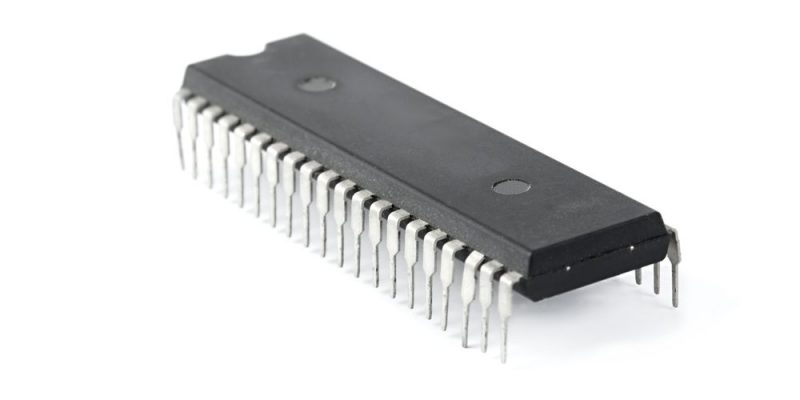
\includegraphics[width=4cm]{rom.jpg}
\centering
\caption{Memoria ROM}
\end{figure}

\subsection{Memoria RAM:}
La Random Access Memory o memoria RAM es una memoria volátil, es decir que una vez se corta el flujo de corriente pierde toda su información. En esta se guardan algunos procesos temporales que el micropocesador debe ejecutar constantemente. Existen diversas variaciones de la memoria RAM, entre estas:
\begin{itemize}
    \item{DRAM (Dynamic RAM)}
    \item{SDRAM (Synchronous DRAM)}
    \item{RDRAM (Rambus DRAM)}
\end{itemize}

\begin{figure}[h]
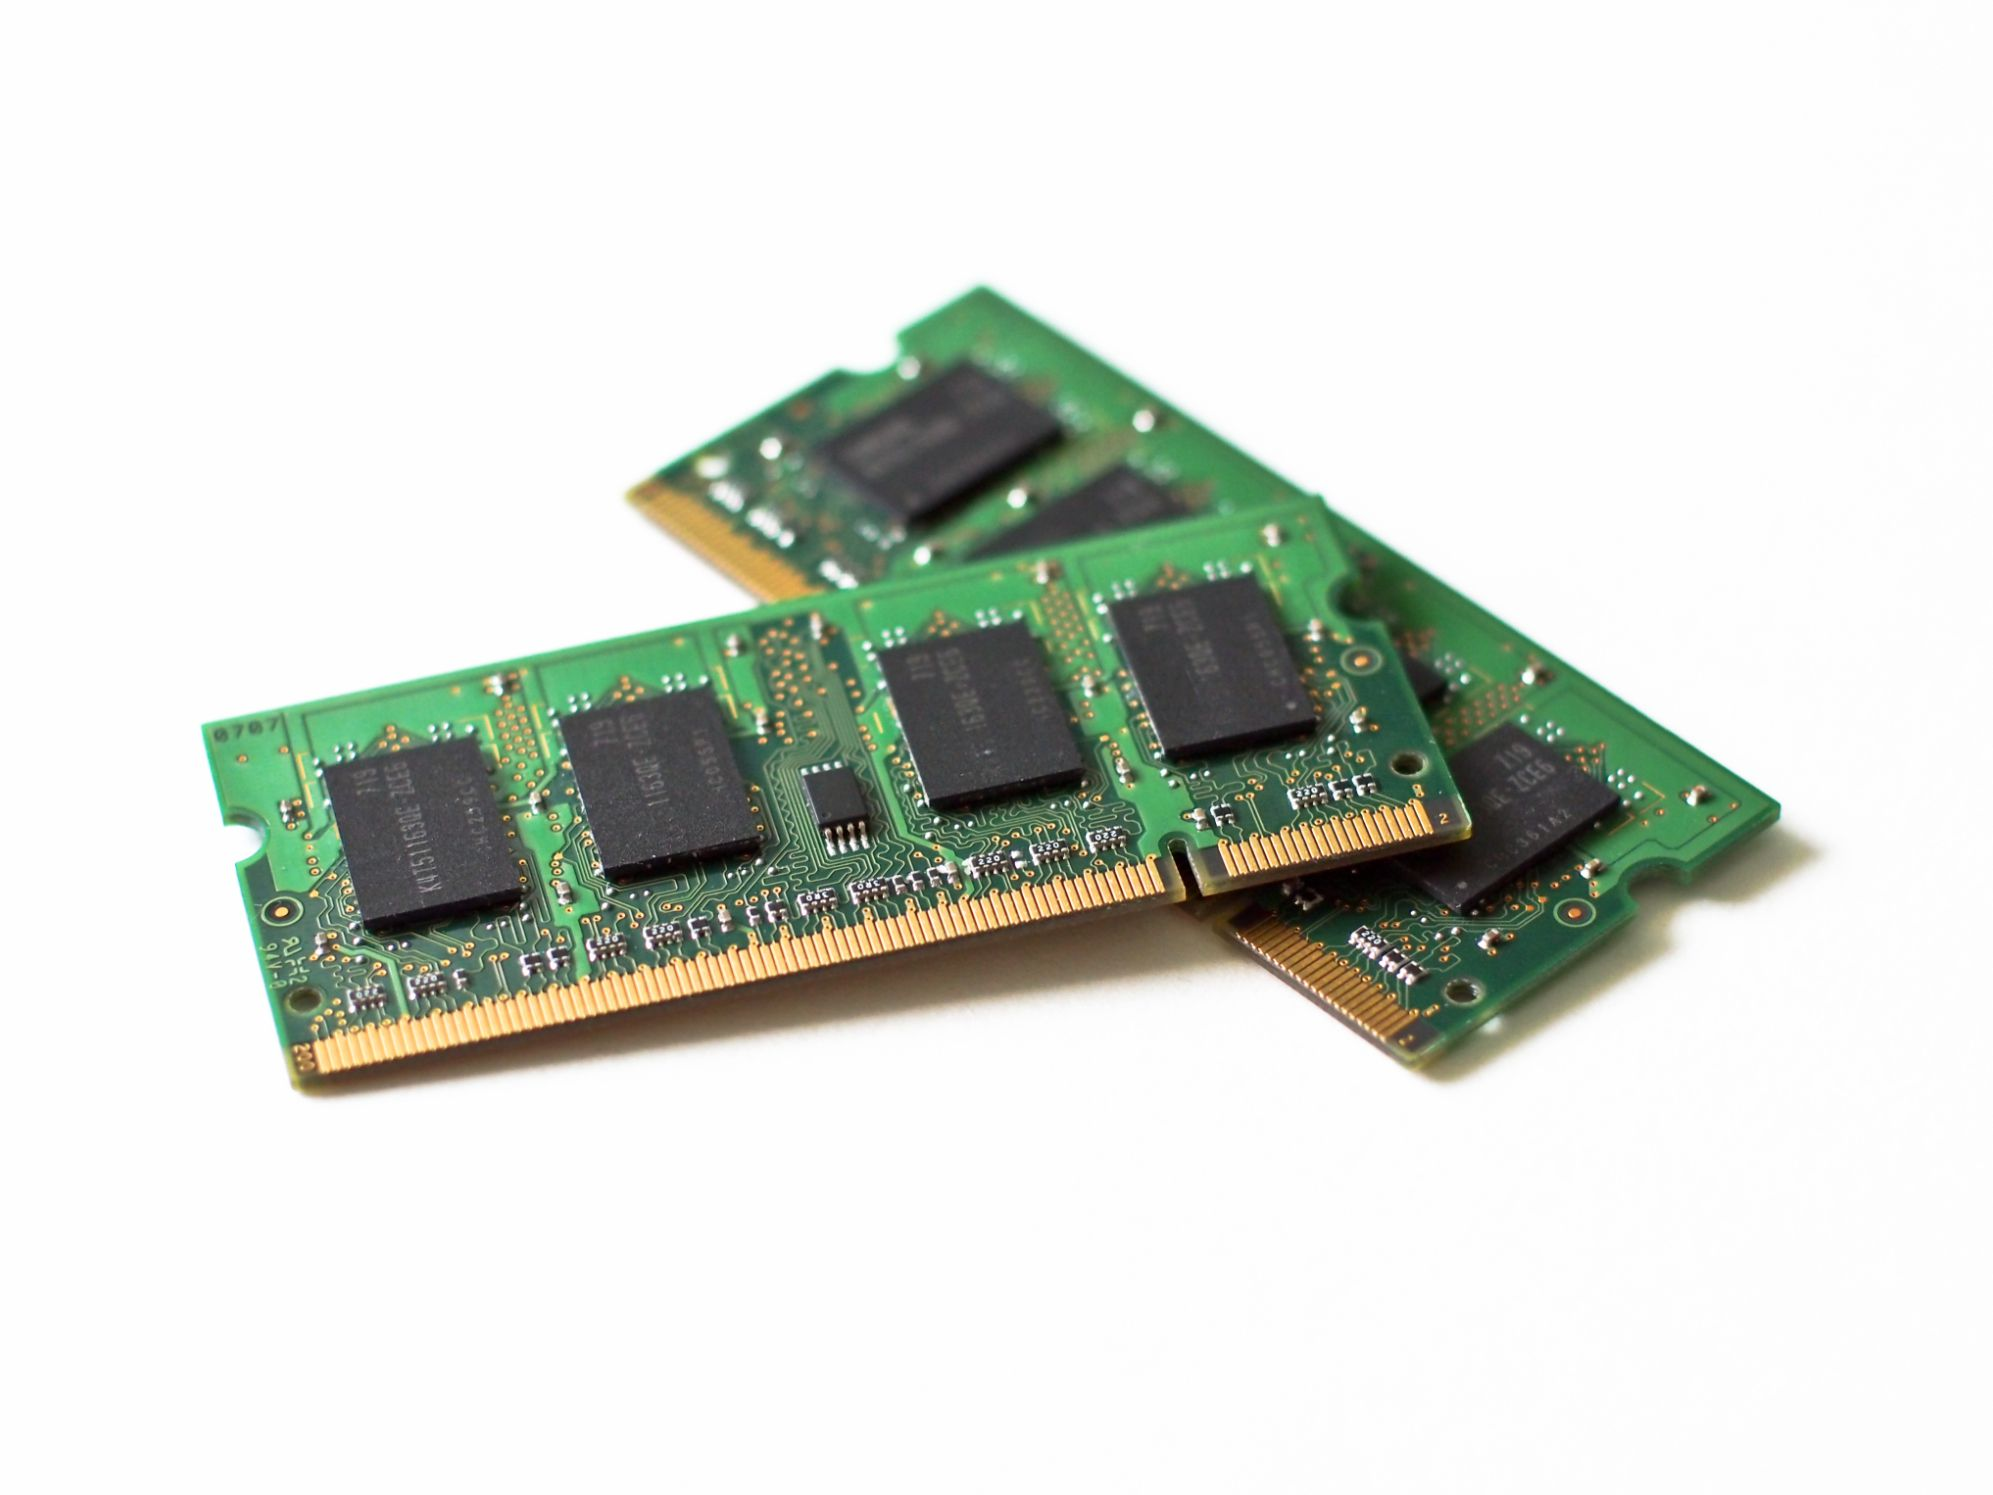
\includegraphics[width=4cm]{memoriaRAM.jpg}
\centering
\caption{Memoria RAM}
\end{figure}

\vfill

\subsection{Memoria Caché: } 
Es una memoria de tipo estático que se sitúa entre el procesador y la memoria principal. Almacena los datos que el procesador debe acceder con más frecuencia para acelerar el acceso a estos. Estas memorias se encuentran divididas en 3 niveles, L1, L2 y L3. El primer nivel de la memoria se encuentra integrado al procesador y por lo tanto el acceso a la información de este nivel es más rápido al de los otros niveles.

\subsection{Disco Duro: } 
El Disco Duro es un dispositivo de almacenamiento que guarda todos los programas y datos de la computadora.  Generalmente se encuentran integrados en la placa base, aunque también existen discos duros externos que se conectan al PC mediante un conector USB. Pueden ser de tipo magnéticos que tienen en su interior varios discos en donde se almacena la información, o pueden ser sólidos en estos no se usan discos giratorios sino matrices de transistores y en cada transistor se guarda una unidad de información.


\section{Gestión de la memoria en un computador}
La memoria del computador se encuentra gestionada por el el MCH (Memory Controller Hub)  que es un circuito integrado que maneja es acceso desde y hacia el microprocesador, la memoria RAM, entre otros. Unas de sus funciones principales es la de controlar el funcionamiento del bus del procesador y la memoria. Un bus es un “conjunto de conexiones físicas (cables, placa de circuito impreso, etc.) que pueden compartirse con múltiples componentes de hardware para que se comuniquen entre sí.”\cite{bus} El bus está dividido en tres subconjuntos:


\subsection{Bus de datos:}
Es de dirección bidireccional y se encarga de transportar los datos procedentes de la memoria con destino al procesador o en dirección opuesta, del procesador a la memoria.

\subsection{bus de direcciones:}
Es de dirección unidireccional y transporta las direcciones de memoria a las que el procesador desea acceder, para la lectura o escritura de datos.

\subsection{bus de control:}
Es de dirección bidireccional y es aquel que gestiona el flujo de información en la memoria que indica si la operación es una lectura o una escritura y la garantía de que la operación ocurre en el momento adecuado.

\section{Velocidad de las memorias e importancia}
Por un lado, la memoria ROM al ser una memoria secuencial debe recorre todos los datos hasta encontrar la información que le es pedida, esto genera demoras en el acceso a la información si la comparamos a la memoria RAM que al ser aleatoria le es posible acceder a los datos de forma directa. Ahora, la memoria caché resulta mucho más rápida que la memoria RAM y por consecuencia de la ROM debido a la inmediatez de esta con el procesador se tiene acceso a la información de esta mucho más rápido que a otras memorias y por esta razón es que es la encargada de almacenar los datos que el procesador necesita de forma más rápida a pesar de la gran diferencia de tamaño con otras memorias.\par
\vspace{5mm}
Por último, leer directamente el disco duro cada que se solicita información resulta en una operación muy larga(se deben recorren los discos para buscar la información), y también es posible que se genere más información que debería guardarse en el proceso, esto requiere más movimiento de información porque lo que lógicamente requerirá más tiempo y aunque la velocidad con la que giran los discos puede hacer el proceso más rápido sigue siendo más rápida una memoria RAM.

La velocidad de una memoria afecta en gran medida el tiempo que le tomará al CPU procesar la información. Una mayor velocidad permite que la transferencia de datos, ya sea almacenar, leer o borrar datos, se realice en menor tiempo y esto en muchos casos genera una diferencia importante en el rendimiento del computador.

\section{Conclusión}
Con esta investigación podemos observar y analizar la importancia que tienen cada uno de los diferentes tipos de memoria y sus usos, podemos tener una idea más clara de como funcionan, en que aspectos se diferencian y como estas diferencias pueden llegar a afectar el rendimiento del computador.

\vspace{5mm}



\bibliographystyle{IEEEtran}
\bibliography{references}
\nocite{*}
\end{document}